\chapter{Introduction}


\section{Dictionaries and Dictionary Learning}
Dictionary models are powerful and versitile tools, useful in denoising \cite{wohlberg2016convolutional}, classification \cite{kong2012dictionary}, anamaly detection \cite{carroll2017outlier}, super-resolution \cite{polatkan2014bayesian}\cite{gu2015convolutional}, inpainting \cite{papyan2017convolutional}, non-rigid struction from motion, and more. Dictionaries are interpretable, and their models are well-suited for incorporating model assumptions using apriori knowledge of the data. In some applications, well-performing dictionaries can be learned from very limited data.

The dictionary model decomposes the signal into the dictionary and coefficients.
%
\begin{equation}
\vs \approx \mD\vx
\end{equation}
%
When the dictionary is known, solving for $\vx$ using $\mD$ and $\vs$ is a pursuit algorithm. When the dictionary is unknown, learning the dictionary from $\vs$ is called dictionary learning. In this dissertation, I present a novel dictionary learning algorithm specifically for convolutional dictionaries.

\subsection{Convolutional Dictionaries}
\begin{figure}
	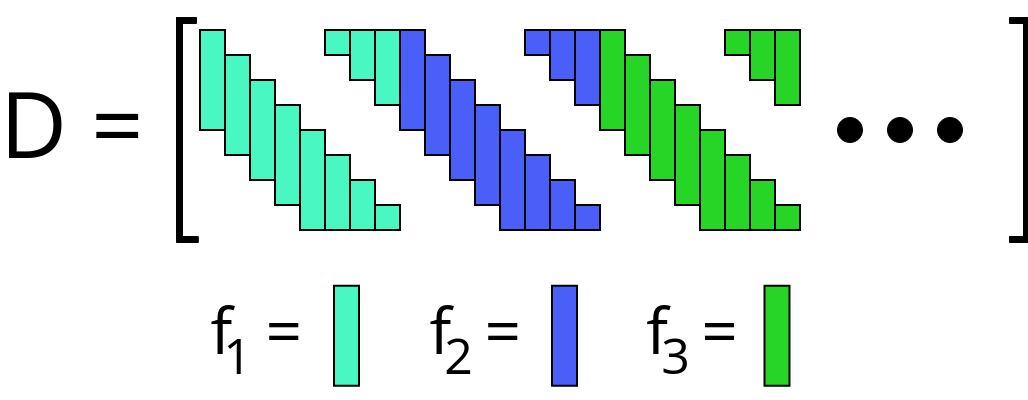
\includegraphics[width=\textwidth]{figures/convolutionalDictionary.png}
	\caption{This is a $1$-dimensional dictionary with convolutional structure. The columns of the dictionary are shifted versions of the dictionary filters.}
	\label{Figure: Convolutional Dictionary}
\end{figure}
The convolutional dictionary model is a dictionary model which imposes a convolutional structure on the dictionary. This structure is shown in figure \ref{Figure: Convolutional Dictionary}. This form of a dictionary can be writen as signals convolved with filters:
\begin{equation}
\vs \approx \sum_i \vf_i * \vx_i
\end{equation}
%
where $\vf_i$ is the $i$th filter of the dictionary, $\vx_i$ is the coefficients for the $i$th filter, and $*$ indicates convolution. This structure is useful for signals where shift-invariance is a desirable characteristic, and often outperforms patch-based methods. For the rest of this dissertation, I will notate $\sum_i \vf_i * \vx_i$ as $\mD\vx$.

\section{Multi-Layer Dictionaries}
A multi-layer dictionary treats the coefficients as the coefficients of a subsequent dictionary model. That is,
\begin{equation}
\vs \approx \mD_1\vx_1
\end{equation}
\begin{equation}
\vx_1 \approx \mD_2\vx_2
\end{equation}
Some researchers have noted that convolutional neural networks resemble multi-layer dictionaries: thresholding is a type of pursuit algorithm, and Rectified Linear Unit activations perform the same operation. A convolutional neural network is a composite function of convolutionals, pooling functions, and activation functions.  Over the last decade, convolutional neural networks have been demonstrated to be highly effective, reaching state-of-the-art performance on a variety of tasks.


\section{Organization of Dissertation}
In chaper $2$, I derive a novel dictionary learning method for multi-channel signals. In chapter $3$, I show how that approach can be adapted to multi-layer dictionary models.  Finally, in chapter $4$ I apply the multi-layer dictionary approach to JPEG compression artifact removal. Chapter $5$ features some practical considerations when implementing these algorithms.

% This is a figure
%\begin{figure}
%	\includegraphics[width=\textwidth]{figures/exampleFigure.png}
%	\caption{This is an example Figure.}
%	\label{Figure in Chapter 1}
%\end{figure}


% This is a table

%\begin{table}
%\caption{This is an example Table.}
%\begin{center}
%\begin{tabular}{ccc}
%x & f(x) & g(x) \\
%\hline
%1 & 6 & 4  \\
%2 & 6 & 3  \\
%3 & 6 & 2  \\
%4 & 6 & 2  \\
%\label{Table in Chapter 1}
%\end{tabular}
%\end{center}
%\end{table}
